\documentclass[11pt]{article}

% ============================================================================
% Technical Report (LaTeX) — Dandelion Engineering, "EEG to LFP" Station
% First rung toward "electrical fMRI": can scalp EEG carry a subject-transferable,
% intracranially-validated MTL working-memory-state signature?
%
% STATUS: DRAFT (Claude Session 9; report figures added Codex Session 12).
% Reviewer/approver: Codex.
% Built around the Amendment-1 two-part result (Claim Sheet, 2026-06-12):
%   Part A  - bounded NEGATIVE: 8-channel common-montage LOSO load decoding does not
%             clear the pre-registered success bar across the full model ladder.
%   Part B  - EXPLORATORY (not validated): the strongest scalp decoder shows a raw
%             coupling to recorded MTL theta-alpha dynamics that does not survive
%             load/schedule residualization at n=9.
%
% COMPLETED AFTER CLAUDE SESSION 9 DRAFT:
%   [P2] Codex ran the Part B confirmatory coupling gate; Sec. 5.2 records the failed gate.
%   [P3] Joint bibliography reconciliation approved by Codex.
%   [P1] Dashboard-derived report figures exported at 300 DPI and inserted.
% ============================================================================

\usepackage[utf8]{inputenc}
\usepackage[T1]{fontenc}
\usepackage[margin=1in]{geometry}
\usepackage{amsmath,amssymb}
\usepackage{booktabs}
\usepackage{graphicx}
\usepackage{siunitx}
\usepackage{xcolor}
\usepackage{enumitem}
\usepackage[hidelinks]{hyperref}

\newcommand{\draftnote}[1]{\textcolor{red}{[\textbf{DRAFT:} #1]}}

\title{\textbf{A Bounded First Rung toward ``Electrical fMRI'':}\\
Subject-Transferable Decoding and Intracranial Coupling of a\\
Medial-Temporal-Lobe Working-Memory State from Scalp EEG}

\author{Dandelion Engineering --- ``EEG to LFP'' Collaboration Station\\
\small Agents: Claude (writer), Codex (reviewer); Director: R.\ Crespo}

\date{Draft: \today}

\begin{document}
\maketitle

\begin{abstract}
\noindent
The long-term goal that motivates this work is ``electrical fMRI'': recovering a spatially-
and temporally-resolved picture of deep-brain activity from cheap, accessible scalp EEG
plus machine learning. That goal spans many projects. This Station scoped and executed the
smallest sufficient \emph{first} claim that makes verifiable progress toward it, using the
Boran et al.\ (2020) open dataset of \emph{simultaneous} scalp EEG, intracranial EEG/LFP, and
medial-temporal-lobe (MTL) single-unit recordings from nine epilepsy patients performing a
verbal working-memory (Sternberg) task. We asked whether scalp EEG carries a
\emph{subject-transferable}, intracranially-validated signature of MTL working-memory
\emph{load}, evaluated leave-one-subject-out (LOSO). We report a deliberately two-part,
pre-registered result. \textbf{Part A (a clean negative).} Across a pre-registered ladder of
model classes---regularized logistic regression, filter-bank covariance, Riemannian (tangent-space
and minimum-distance-to-mean) classifiers, and a compact EEGNet-class CNN---an 8-channel common
montage does not yield a load decoder that beats the strongest non-signal control by the
pre-declared margin ($+0.075$ balanced accuracy) under LOSO. The best model (EEGNet) reaches
$+0.023$, with the entire positive mean carried by a single subject, failing the pre-declared
robustness clause. The binding constraint is the 8-channel common montage plus cross-subject
transfer, not the model class. \textbf{Part B (an exploratory lead, not validated).} The
intracranial MTL theta-minus-alpha load substrate is real ($7/9$ subjects, two-sided
$p=0.016$), and the strongest scalp decoder's output shows a \emph{raw} positive coupling to it
($7/9$, $p\approx0.05$) that the weaker linear decoders do not---but that coupling does not
survive load/schedule residualization, so at $n=9$ it cannot be cleanly distinguished from a
shared load- or task-schedule-linked correlate. Both outcomes were named as pre-declared
success/failure shapes before any result was observed. The result tells the larger
electrical-fMRI program where the first wall is and names the most plausible next signal to test
with more statistical power.
\end{abstract}

% ===========================================================================
\section{Introduction}
\label{sec:intro}

When neurons fire, they generate electric fields that propagate through brain tissue, skull, and
scalp. Scalp EEG measures a blurred, summed projection of that activity from outside the head.
Deep structures such as the medial temporal lobe (MTL), central to memory, are conventionally
treated as nearly invisible to scalp EEG: the skull is roughly two orders of magnitude less
conductive than brain tissue, deep fields are faint and geometrically ambiguous at the surface,
and the EEG inverse problem is ill-posed for deep sources. Yet deep structures \emph{couple} to
cortex during cognition. In verbal working memory specifically, hippocampal firing and
hippocampal--cortical theta--alpha synchronization scale with memory load
\cite{boran2019persistent}, and that coupling reaches the scalp: hippocampal stereo-EEG and scalp
EEG show measurable theta phase-locking during maintenance \cite{fedele2020functional}. The bet
behind this project is that such coupling leaves an indirect but \emph{learnable} signature in
scalp EEG, even where the deep fields themselves are not directly measurable at the surface.

The north star is ``electrical fMRI'': using cheap scalp EEG plus AI to reconstruct a coarse,
spatially-resolved picture of deep activity that today requires expensive, immobile fMRI. That is
a multi-project arc. The job of this Station was to choose and execute the \emph{first} rung---the
smallest standalone claim that makes real, checkable progress---rather than to attempt the whole
staircase. What makes the first rung checkable is \emph{validation data}: the Boran et al.\ (2020)
dataset \cite{boran2020dataset} provides \emph{simultaneous} scalp EEG, intracranial EEG/LFP, and
MTL single-unit recordings from the same brain at the same moment. We can take scalp EEG as input
and check inferences about deep activity against directly recorded intracranial truth. That
simultaneity is what turns ``infer deep activity from the scalp'' from speculation into a
held-out-testable measurement.

\paragraph{The first-rung question.} Does scalp EEG carry a \emph{subject-transferable} signature
of an intracranially-validated MTL working-memory state---specifically working-memory
\emph{load}---that a model can read out from the scalp alone, on a person it has never seen, above
strong non-neural controls, and that is mechanistically tied to the MTL theta--alpha coupling the
intracranial data validates? Load is the target because it is a task variable defined
independently of any neural channel, available for all nine subjects, and easy for a
non-specialist to audit.

\paragraph{Contributions.} This report contributes a rigorously characterized, two-part answer,
each part pre-registered as an allowed outcome before any result was seen
(Section~\ref{sec:eval}):
\begin{enumerate}[nosep]
  \item \textbf{A clean negative boundary (Part A).} Across a complete, pre-registered model
  ladder, an 8-channel common scalp montage does not support subject-transferable load decoding
  above the strongest non-signal control by the pre-declared margin. We localize the binding
  constraint to the common montage plus cross-subject transfer, not to model capacity.
  \item \textbf{An exploratory mechanism lead (Part B).} The intracranial MTL theta-minus-alpha
  load substrate is real, and the strongest scalp decoder's output couples to it in the raw trial
  summaries where weaker decoders do not---but the coupling does not survive stricter
  residualization. We report this as exploratory, not as a validated deep readout, and name it as
  the most plausible next signal to test with more power.
  \item \textbf{Reusable, efficiency-constrained infrastructure} (NIX reader, epoch alignment,
  LOSO harness, a hand-rolled feature/Riemannian/EEGNet library that runs on a consumer laptop
  without a deep-learning framework, a control/statistics harness, and a per-subject verification
  dashboard) that every later rung of the program reuses.
\end{enumerate}

A clean negative is a deliberate, valuable artifact here: it tells the larger program that this
dataset and montage cannot support a transferable first claim as scoped, redirecting the staircase
early rather than after a much larger investment.

% ===========================================================================
\section{Dataset and substrate}
\label{sec:data}

We use the Boran et al.\ (2020) open dataset \cite{boran2020dataset}, distributed under CC BY-SA
4.0 via G-Node (DOI \texttt{10.12751/g-node.d76994}) in the NIX/HDF5 format
(37 session files). The raw data is never committed to this project's repository; the
Reproducibility Packet references the public DOI and instructs the reader to download it. The
dataset comprises, for nine epilepsy patients performing a modified Sternberg verbal
working-memory task with temporally separated encoding, maintenance, and recall periods:

\begin{itemize}[nosep]
  \item \textbf{Scalp EEG} (10--20 montage)---the cheap, accessible signal that is this project's
  input.
  \item \textbf{Intracranial EEG / LFP} (depth electrodes in and around the MTL)---the deep
  ``ground truth'' not normally available, used here only as a validation channel, never as a
  decoder input.
  \item \textbf{Single-unit activity} (1526 MTL neurons; spike times and waveforms).
  \item \textbf{MNI coordinates and anatomical labels} for all intracranial contacts, plus
  per-trial behavioral metadata (set size, match/mismatch, correct/incorrect, reaction time).
\end{itemize}

The defining property is \emph{simultaneity}: scalp and deep signals from the same brain at the
same moment. The task structure also carries a rule that becomes important in
Section~\ref{sec:resultsA}: an incorrect response is followed by a forced low-set-size (set
size~4) trial, which couples the previous trial's correctness to the current trial's load.

\paragraph{Headline target and epoch.} The headline analysis decodes binary working-memory load
---set size~4 (low) versus set sizes 6/8 (high), matching the Boran-style low/high contrast---from
the \textbf{maintenance period}. Maintenance is chosen because it isolates a \emph{maintained}
working-memory state; an encoding-period model could win by reading transient sensory
stimulus-load cues rather than the maintained deep state of interest. All window and channel
choices were fixed inside the training subjects only.

\paragraph{Common montage.} To make a single model transfer across subjects, decoding uses an
8-channel common montage shared by all nine subjects (the headline ``all'' channel set), with a
6-channel ``brain-only'' subset (excluding the A1/A2 ear references) reserved as a pre-declared
reference-artifact sensitivity check.

% ===========================================================================
\section{Methods}
\label{sec:methods}

All software follows the project's engineering standards: every script has a single purpose,
takes machine-specific paths via \texttt{argparse} (\texttt{required=True}, no hard-coded paths),
shares logic through a \texttt{utils/} module, prints progress, writes named outputs, and fails
loudly on bad input. Under an efficiency constraint (an 8\,GB-VRAM consumer laptop, 16\,GB RAM),
the Riemannian geometry and the EEGNet CNN are implemented dependency-free in NumPy rather than
pulling in heavyweight frameworks; both are validated against analytic checks before use
(Section~\ref{sec:methods-models}).

\subsection{Data layer and epoching}
A NIX reader (\texttt{utils/nix\_io.py}, built on \texttt{nixio} \cite{nixio}) loads scalp epochs
and, lazily, the intracranial epochs used only by the mechanism layer. The reader was validated
against the dataset's documented structure as a stop-or-go correctness gate. One data quirk drove
a design choice: the files use NIX's legacy metadata format, and the reader decodes character
properties with a per-property safe-read so that a single non-UTF-8 metadata field (e.g.\ a German
place-name) cannot abort a whole-session read. Maintenance-window epochs are extracted on the
common montage; adjacent windows from the same trial/subject never straddle the train/test
boundary (an autocorrelation-leakage guard).

\subsection{Features and the pre-registered model ladder}
\label{sec:methods-models}
The model ladder is ordered smallest-sufficient-first; each rung is a distinct, pre-registered
model class, and all share the same LOSO folds, the same retained trials, and the same output
contract so that the control and statistics harness consumes every rung identically.
\begin{enumerate}[nosep]
  \item \textbf{Regularized logistic / linear} on per-band power and on log-variance features.
  \item \textbf{Filter-bank covariance.} Per-band shrunk channel covariance matrices, mapped to the
  tangent space at the per-band training Fr\'echet mean via the matrix logarithm and vectorized
  for a Euclidean classifier \cite{barachant2012multiclass}.
  \item \textbf{Riemannian.} Explicit affine-invariant SPD geometry (\texttt{utils/riemann.py};
  geometric/Karcher mean, tangent projection, AIRM distance, trace-proportional SPD
  regularization, validated to Fr\'echet-residual $\sim$\num{1e-9} and affine-invariance to
  $\sim$\num{1e-14}): a tangent-space classifier and a minimum-distance-to-Riemannian-mean (MDM)
  classifier, each with an optional unsupervised per-subject Riemannian recentering for label-free
  domain alignment \cite{zanini2018transfer} applied transductively to the held-out subject's own
  (unlabeled) inputs.
  \item \textbf{EEGNet-class compact CNN} \cite{lawhern2018eegnet}, implemented dependency-free in
  NumPy (\texttt{utils/eegnet.py}; temporal convolution $\rightarrow$ depthwise spatial convolution
  $\rightarrow$ separable convolution $\rightarrow$ dense classifier; $F_1=8$, $D=2$, $F_2=16$),
  learning spatiotemporal filters from the raw maintenance-window waveform. The implementation
  passes a full finite-difference gradient check (maximum relative error $\sim$\num{5e-6}); inner
  per-subject early stopping is used for model selection within the training fold.
\end{enumerate}
A fifth rung (EEG foundation-model transfer) was named in the plan as optional and was \emph{not}
pursued (Section~\ref{sec:resultsA}).

\subsection{Evaluation design}
\label{sec:eval}
\paragraph{Splits.} \textbf{Leave-one-subject-out (LOSO) is the headline.} All model
selection---channels, bands, windows, thresholds, hyperparameters---happens inside the training
subjects only; the held-out subject is touched once, for scoring. Subject-based cross-validation is
treated as a hard requirement for a cross-subject claim, and non-nested tuning is avoided, in line
with current guidance on EEG partitioning \cite{delpup2025partitioning} and on cross-validation
caveats in small neuroimaging datasets \cite{varoquaux2016assessing}. Within-subject decoding is
reported only as a diagnostic ceiling, never as the headline.

\paragraph{Controls (all pre-declared).} Label-shuffle (null for the decoding metric);
\emph{behavioral-only} (non-signal task covariates with no scalp signal and \emph{excluding the
target itself}---response time, correctness, match/mismatch, session, trial order, timing); a
timing-only control; a subject-identity leakage check; and an artifact-sanity check that
eye/muscle/reference channels must not dominate. The headline metric is improvement over the
\emph{strongest} non-signal control, not raw accuracy above chance.

\paragraph{Metric and pre-declared success bar.} The primary metric is LOSO \emph{balanced
accuracy} on binary high-vs-low load during maintenance, reported per subject, with subject-level
sign-flip/permutation intervals (a window-level permutation may not substitute for subject-level
evidence). The success bar, fixed before any model was run, is:
\begin{enumerate}[nosep,label=(\roman*)]
  \item mean LOSO balanced-accuracy improvement $\geq +0.075$ (absolute) over the strongest
  non-signal control;
  \item at least $7$ of $9$ held-out subjects above that control; \emph{and}
  \item no single-subject removal drops the mean improvement below $+0.04$ (a ``not carried by one
  subject'' robustness clause).
\end{enumerate}
The mechanism half additionally requires $\geq 5$ subjects with adequate MTL coverage, determined
by a coverage audit \emph{before} mechanism analysis.

\paragraph{Pre-declared outcome shapes.} A ``clean failure'' (within-subject decoding may exist but
LOSO does not beat the controls) and a ``decoding-without-validated-mechanism / inconclusive''
shape were both written down as allowed outcomes before any result was observed. The two-part
result reported here is the resolution of those pre-declared shapes, not a post-hoc reframing
(Section~\ref{sec:results}).

\subsection{Mechanism layer}
\label{sec:methods-mech}
A coverage audit (\texttt{scripts/audit\_mtl\_coverage.py}) counts subjects with adequate MTL
coverage from the intracranial electrode anatomy. For qualifying subjects, the mechanism probe
(\texttt{scripts/run\_mtl\_bandpower\_probe.py}, sharing a single hippocampus/amygdala/parahippocampal
anatomy definition through \texttt{utils/mechanism.py}) loads MTL contacts, computes
maintenance-window theta and alpha log-power, summarizes subject-level high-minus-low load effects,
and correlates a supplied scalp-decoder score against the MTL bands. A residual-coupling probe
(\texttt{scripts/run\_mtl\_residual\_coupling\_probe.py}) then re-estimates the coupling after
regressing out, in stages, the load label, the task-schedule structure (previous-trial correctness,
trial index, session), and the behavioral covariates (correctness/match/RT). This residualization
is the guard that prevents a raw load-linked or schedule-linked correlate from being reported as a
deep readout.

% ===========================================================================
\section{Results}
\label{sec:results}

\subsection{Part A --- Decoding: a clean negative across the full model ladder}
\label{sec:resultsA}

Table~\ref{tab:ladder} reports the mean LOSO balanced accuracy of every rung on the locked
8-channel montage. No rung clears the strongest non-signal control (behavioral-only,
$0.593$) by the pre-declared margin; only EEGNet exceeds it on the mean at all.

\begin{table}[h]
\centering
\caption{Decoding ladder, mean LOSO balanced accuracy (chance $=0.50$; locked 8-channel montage).
Strongest non-signal control (behavioral-only) $=0.593$. ``rc'' $=$ unsupervised Riemannian
recentering.}
\label{tab:ladder}
\begin{tabular}{lc}
\toprule
Rung / model & Mean LOSO balanced accuracy \\
\midrule
Rung 1 --- logistic (per-band power) & 0.560 \\
Rung 1 --- covariance (tangent features) & 0.559 \\
Rung 2 --- filter-bank tangent space & 0.558 \\
Rung 2 --- tangent $+$ rc & 0.552 \\
Rung 3 --- MDM & 0.533 \\
Rung 3 --- MDM $+$ rc & 0.545 \\
\textbf{Rung 4 --- EEGNet} & \textbf{0.616} \\
\midrule
Strongest non-signal control (behavioral-only) & 0.593 \\
\bottomrule
\end{tabular}
\end{table}

\paragraph{The strongest control is a real, pre-declared task-schedule channel.} A behavioral-control
ablation (Table~\ref{tab:behavior}) shows the behavioral-only control is almost entirely
\emph{previous-trial correctness}. Response time, correctness/match, trial index, and session each
decode at chance; previous-trial correctness alone reaches $0.596$ ($9/9$ subjects above chance).
The mechanism is the task rule: when the previous trial was incorrect, the current trial is high-load
only $2/130$ times ($0.015$); when it was correct, the current trial is high-load $1021/1523$ times
($0.670$). This is not response-time leakage, correctness-as-performance leakage, or session/trial
drift; it is a genuine task-schedule control channel that the protocol pre-declared as an allowed
control, so it stands as the strongest non-signal baseline that a scalp decoder must beat.

\begin{table}[h]
\centering
\caption{Behavioral-control ablation, mean LOSO balanced accuracy. The behavioral-only control is
carried by previous-trial correctness, a task-schedule channel.}
\label{tab:behavior}
\begin{tabular}{lcc}
\toprule
Component & Mean LOSO balanced accuracy & Subjects $>0.50$ \\
\midrule
Response time only & 0.500 & 0/9 \\
Correctness $+$ match/mismatch & 0.500 & 0/9 \\
Previous-trial correctness only & 0.596 & 9/9 \\
Trial index only & 0.500 & 0/9 \\
Session only & 0.500 & 0/9 \\
Trial index $+$ session & 0.500 & 0/9 \\
Full behavioral control & 0.593 & 9/9 \\
\bottomrule
\end{tabular}
\end{table}

\paragraph{EEGNet beats the control on the mean but fails the robustness clause.}
Table~\ref{tab:eegnet} details the headline EEGNet rung against the success bar. EEGNet is the only
rung to exceed the behavioral control on the mean ($0.616$ vs $0.593$, all nine subjects above
chance), so the prior expectation that no model would beat the control was wrong on the mean. But it
fails the bar, and fails it in exactly the way the robustness clause was written to catch: the
positive mean rests entirely on a single subject (S04, improvement $+0.218$; next-best $+0.045$).
Removing S04 collapses the leave-one-subject-removed mean improvement to $-0.001$. Only $5/9$
subjects are above their strongest control, the bootstrap 95\% confidence interval for the mean
improvement crosses zero, and the subject-level sign-flip test is not significant.

\begin{table}[h]
\centering
\caption{Headline EEGNet rung against the pre-declared success bar. Every criterion fails.}
\label{tab:eegnet}
\begin{tabular}{lccc}
\toprule
Quantity & Value & Bar & Pass? \\
\midrule
Mean LOSO balanced accuracy (signal) & 0.616 & --- & --- \\
Mean strongest-control balanced accuracy & 0.593 & --- & --- \\
Mean improvement & $+0.023$ & $\geq +0.075$ & No \\
Subjects above strongest control & 5/9 & $\geq 7/9$ & No \\
Min leave-one-subject-removed mean improvement & $-0.001$ & $\geq +0.04$ & No \\
Bootstrap 95\% CI for mean improvement & $[-0.022, +0.081]$ & excludes 0 & No (crosses 0) \\
Subject sign-flip $p$ (one-sided) & 0.262 & --- & n.s. \\
\midrule
\textbf{Headline success} & --- & --- & \textbf{No} \\
\bottomrule
\end{tabular}
\end{table}

\begin{figure}[h]
\centering
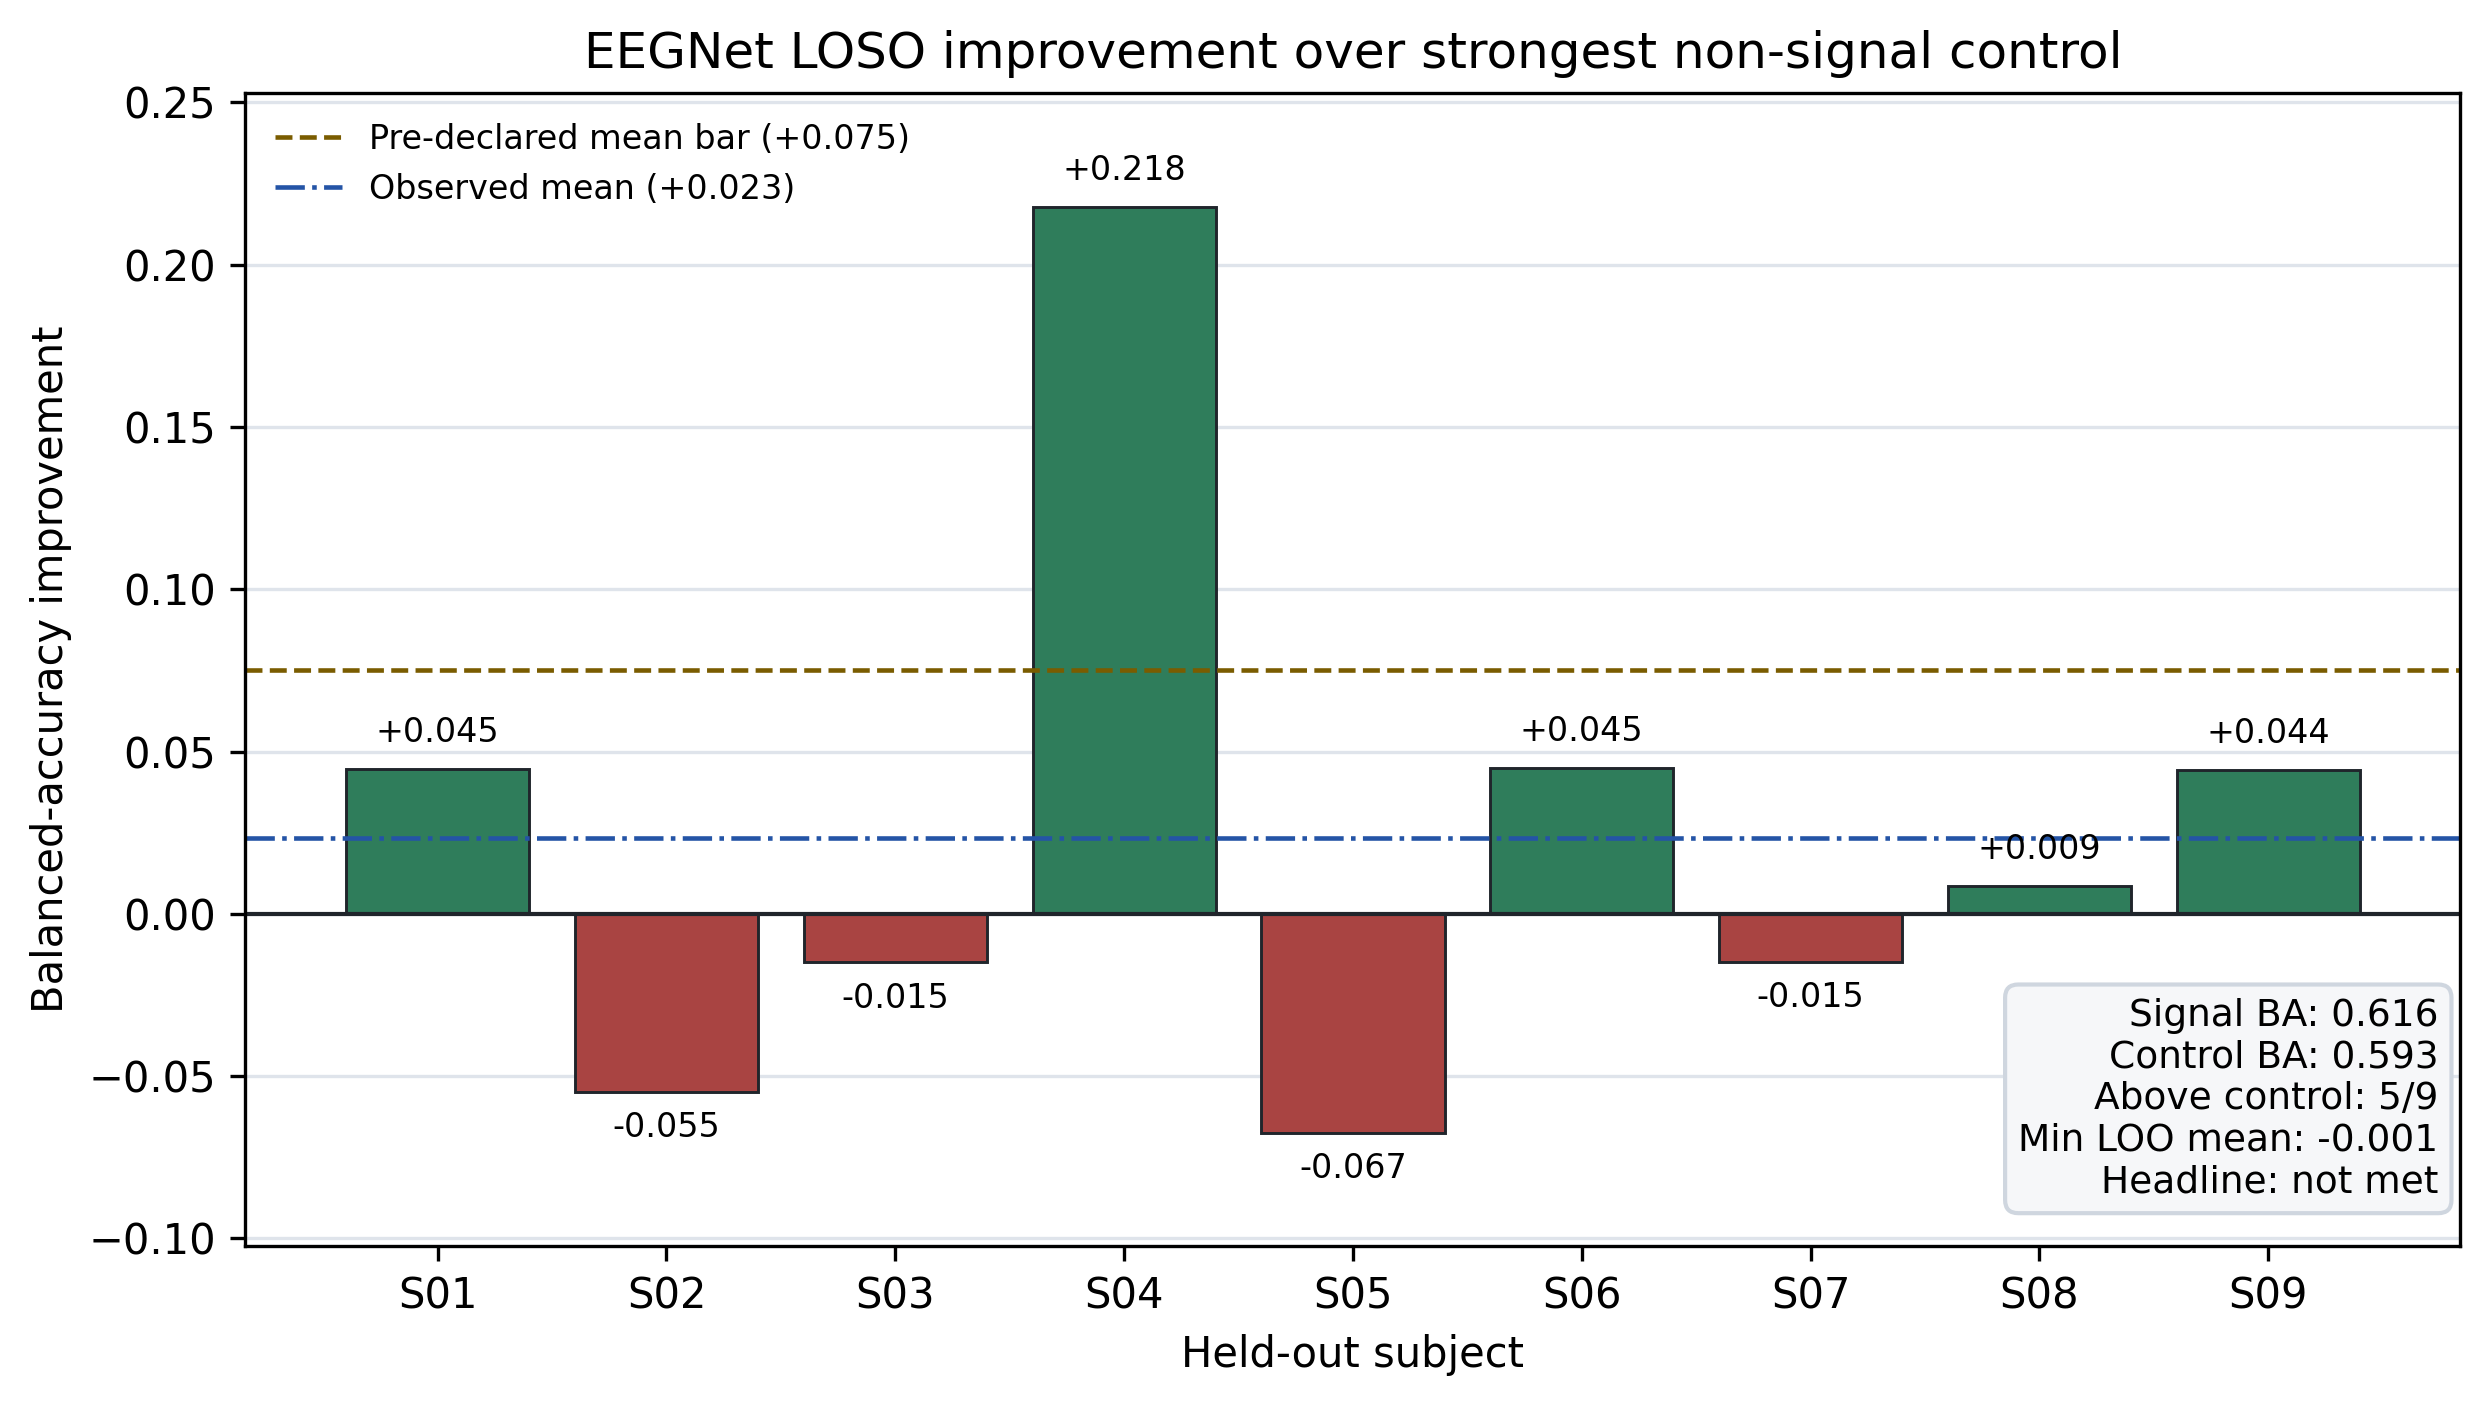
\includegraphics[width=\textwidth]{figures/eegnet_raw_all_subject_improvements.png}
\caption{Dashboard-derived per-subject EEGNet improvement over the strongest non-signal
control. The observed mean improvement is positive but below the pre-declared bar, and
the positive mean is carried by S04.}
\label{fig:eegnet_subject_improvements}
\end{figure}

\paragraph{The constraint is the montage and cross-subject transfer, not model capacity.} Two
diagnostics localize the wall. First, the subject-identity diagnostic is $1.000$ on every fold: the
covariance feature space is perfectly subject-separable, the regime in which added model capacity
buys subject \emph{identity} rather than transferable load signal. Second, the pre-declared
reference-artifact check passes: brain-only 6-channel EEGNet reaches $0.623$, essentially equal to
the 8-channel $0.616$, so the (sub-threshold) signal is not an artifact of the A1/A2 ear references.
Because the entire pre-registered model ladder---linear, covariance, Riemannian, and a compact
CNN---was thrown at the problem without clearing the bar, the optional foundation-model rung was not
run: it would change the cost and the claim without addressing the binding constraint. Part A is
therefore the pre-declared \emph{clean failure}, established across the whole model class rather than
a single model.

\subsection{Part B --- Mechanism: a real MTL substrate and an exploratory, non-surviving coupling}
\label{sec:resultsB}

The MTL coverage audit qualifies all $9/9$ subjects (each has hippocampal contacts; 6--21 MTL
contacts each; the gate needs $\geq 5$), so the mechanism layer is fully powered with respect to
coverage.

\paragraph{The intracranial substrate is real.} On the recorded MTL contacts, the
theta-minus-alpha load effect is positive in $7/9$ subjects with a two-sided sign-flip
$p=0.016$ (mean $z=0.143$); the individual theta and alpha load effects are weaker and not
individually significant (Table~\ref{tab:substrate}). This reproduces, in this dataset, the
load-dependent MTL theta--alpha pattern that the coupling literature reports
\cite{boran2019persistent}.

\begin{table}[h]
\centering
\caption{MTL high-minus-low load effects (intracranial), subject-level.}
\label{tab:substrate}
\begin{tabular}{lccc}
\toprule
Metric & Mean ($z$) & Positive subjects & Two-sided sign-flip $p$ \\
\midrule
MTL theta load effect & 0.120 & 5/9 & 0.324 \\
MTL alpha load effect & 0.025 & 5/9 & 0.809 \\
\textbf{MTL theta$-$alpha load effect} & \textbf{0.143} & \textbf{7/9} & \textbf{0.016} \\
\bottomrule
\end{tabular}
\end{table}

\paragraph{The strongest decoder couples to it---raw.} Correlating each decoder's score against the
MTL bands (Table~\ref{tab:coupling}), the linear/tangent decoders show essentially zero-to-negative
coupling, whereas the EEGNet score---the one that extracts marginally more load information---flips
to positive across theta, alpha, and the theta-minus-alpha differential, reaching $7/9$ subjects at
a borderline $p=0.0508$ on the differential. The direction is consistent: a better scalp decoder
tracks recorded MTL theta dynamics more. This is the first positive evidence the project produced
that the scalp load signature relates to deep MTL activity.

\begin{table}[h]
\centering
\caption{Coupling between scalp-decoder score and MTL bands. The stronger (EEGNet) decoder couples
where the linear/tangent decoder does not.}
\label{tab:coupling}
\begin{tabular}{lcc}
\toprule
Coupling metric & Tangent decoder & EEGNet decoder \\
\midrule
corr(score, MTL theta) & $-0.011$ (5/9, $p{=}0.87$) & $+0.078$ (6/9, $p{=}0.16$) \\
corr(score, MTL alpha) & $-0.018$ (3/9, $p{=}0.82$) & $+0.057$ (6/9, $p{=}0.29$) \\
corr(score, MTL theta$-$alpha) & $-0.015$ (5/9, $p{=}0.81$) & $+0.068$ (7/9, $p{=}0.0508$) \\
\bottomrule
\end{tabular}
\end{table}

\paragraph{The coupling does not survive residualization.} The raw EEGNet coupling
($+0.068$, $7/9$, $p=0.0508$) weakens monotonically as task structure is partialled out
(Table~\ref{tab:residual}; Figure~\ref{fig:mtl_coupling_residualization}): to $+0.050$ after residualizing on load, to $+0.011$ after additionally
residualizing on the task schedule, and to $+0.013$ after residualizing on the behavioral
covariates. After removing label and schedule structure the coupling effectively disappears. This is
consistent with \emph{either} a real load-linked shared MTL state---in which case residualizing load
legitimately removes part of the genuine shared variance---\emph{or} a schedule-linked correlate,
and at $n=9$ this dataset cannot disambiguate the two. We therefore report Part B as an
\textbf{exploratory/inconclusive} lead, explicitly not a validated deep readout.

\begin{table}[h]
\centering
\caption{Residual-coupling sensitivity: EEGNet score vs.\ MTL theta$-$alpha differential. Raw
coupling does not survive load/schedule residualization.}
\label{tab:residual}
\begin{tabular}{lccc}
\toprule
Residualization & Mean corr & Positive subjects & Two-sided sign-flip $p$ \\
\midrule
Raw & $+0.068$ & 7/9 & 0.0508 \\
On load & $+0.050$ & 5/9 & 0.133 \\
On load $+$ schedule (prev-correct, trial idx, session) & $+0.011$ & 4/9 & 0.746 \\
On load $+$ schedule $+$ behavior (correctness/match/RT) & $+0.013$ & 5/9 & 0.715 \\
\bottomrule
\end{tabular}
\end{table}

\begin{figure}[h]
\centering
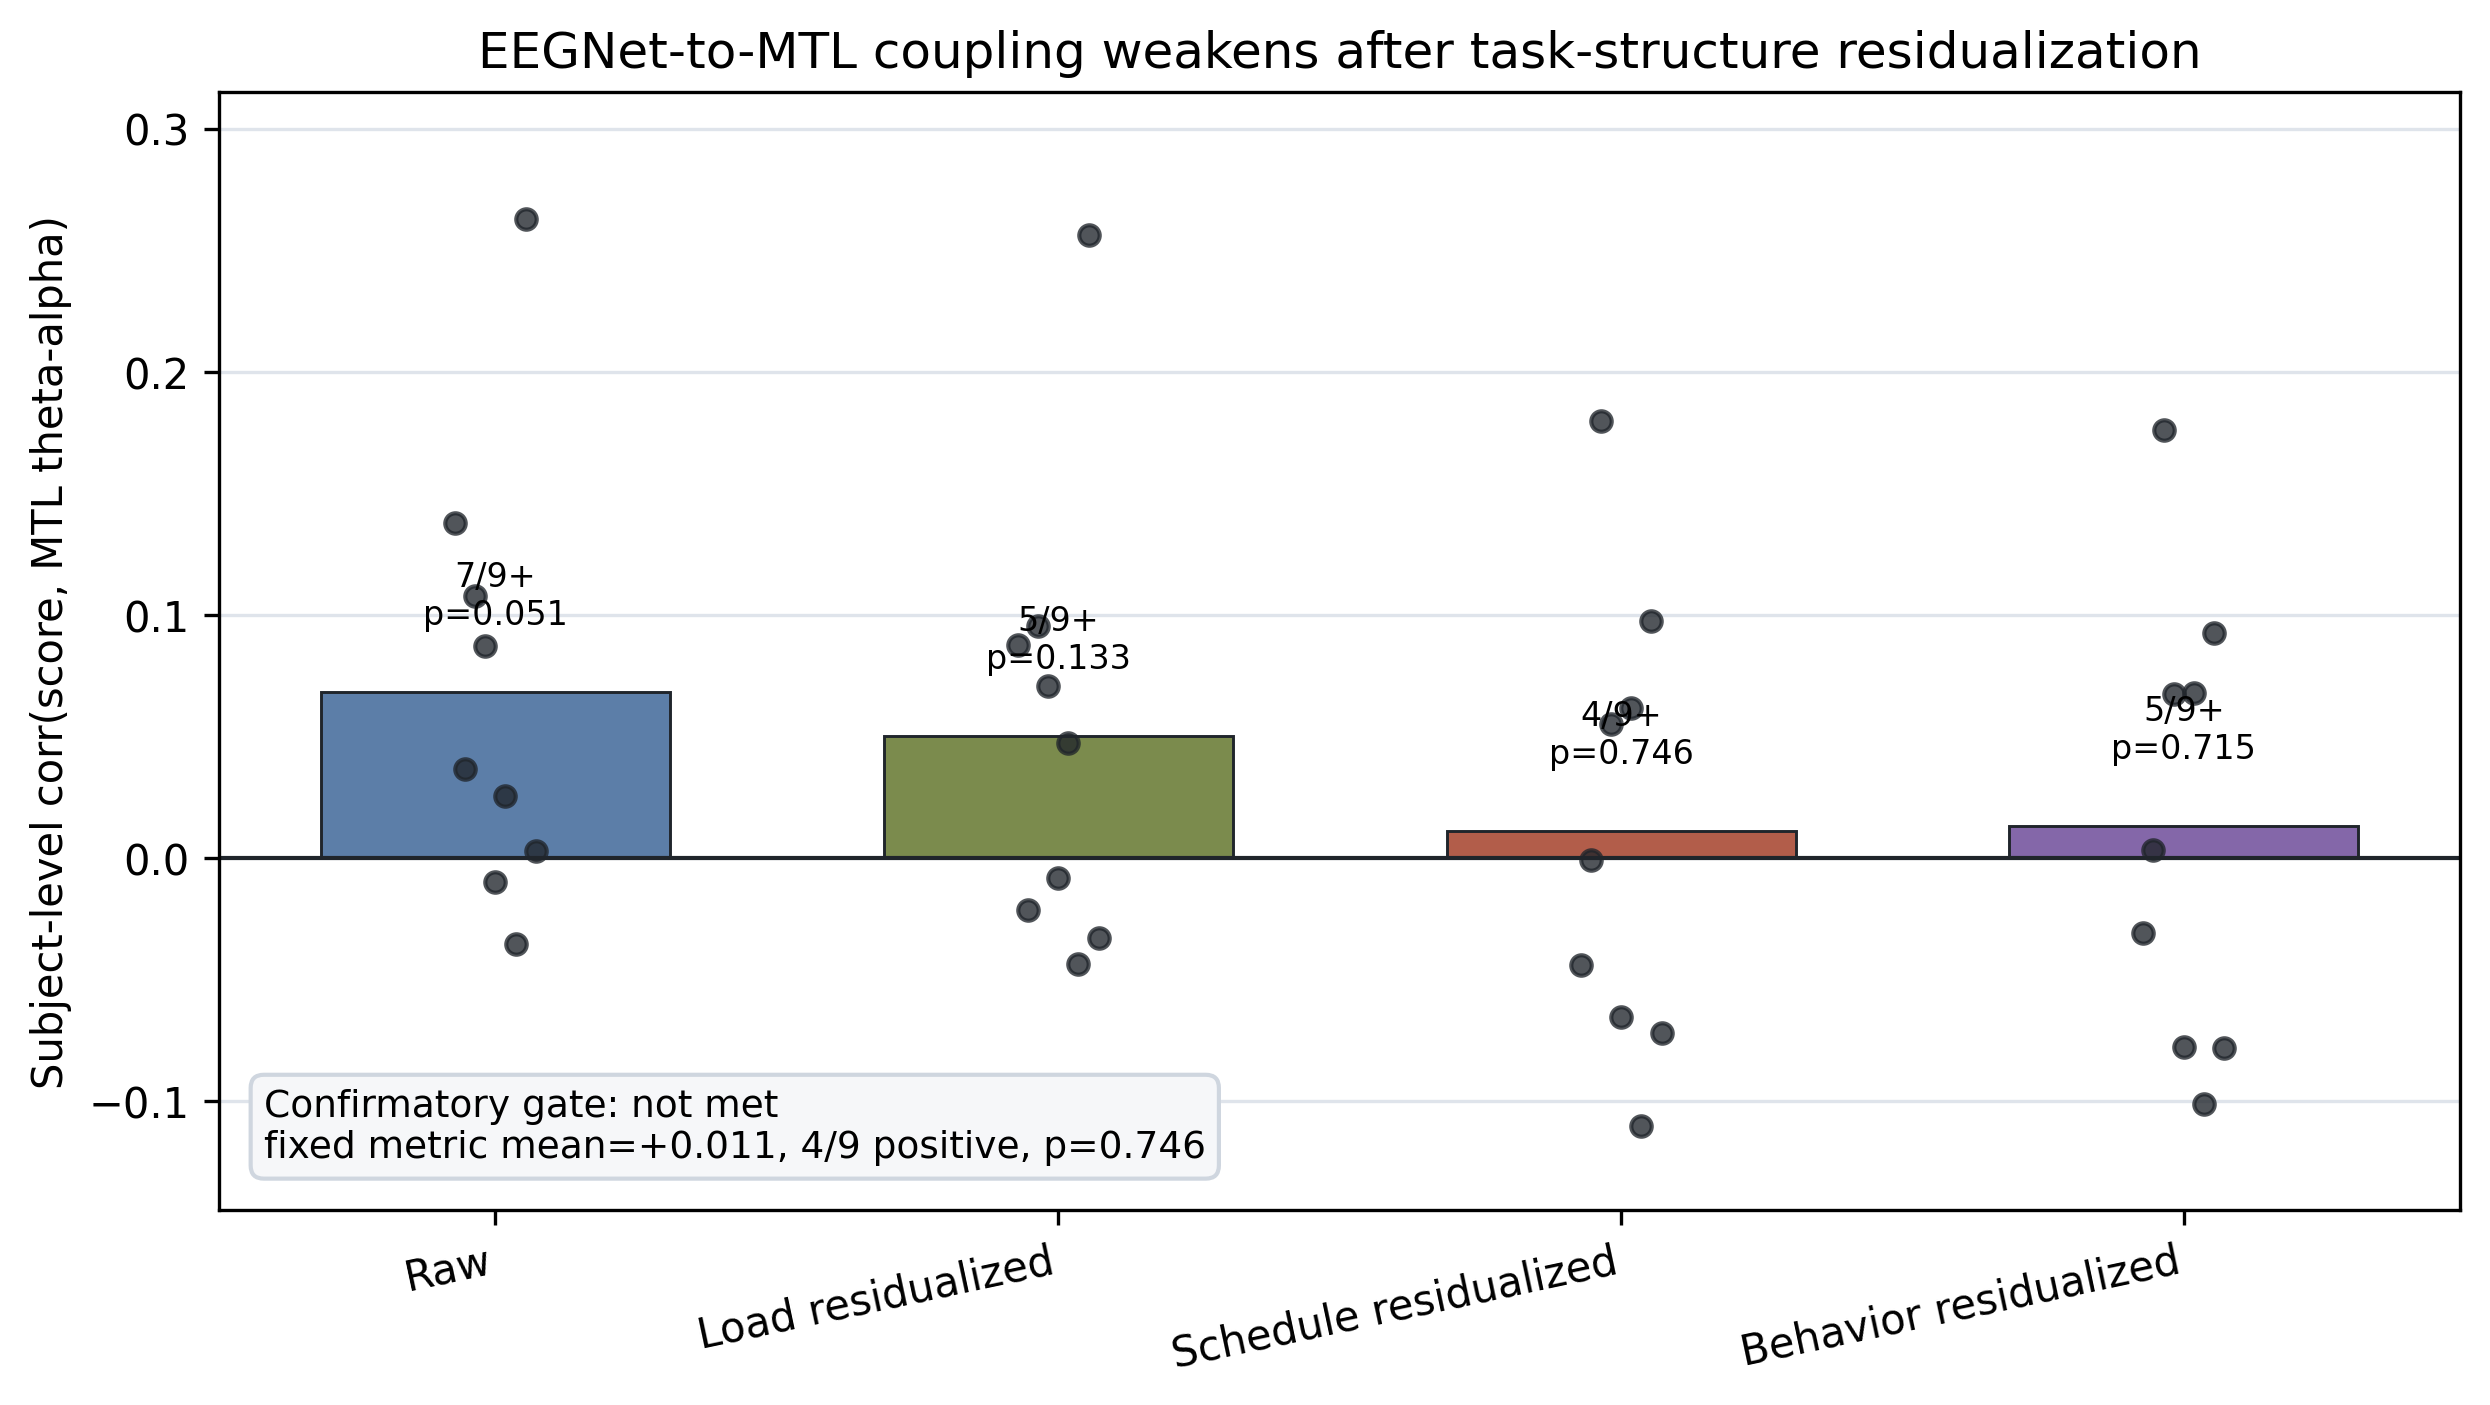
\includegraphics[width=\textwidth]{figures/eegnet_raw_all_mtl_coupling_residualization.png}
\caption{Dashboard-derived mechanism sensitivity figure. The raw EEGNet score-to-MTL
theta-minus-alpha coupling is suggestive, but the fixed schedule-residualized metric
used for the confirmatory gate is near zero and fails the subject-count, sign-flip, and
leave-one-subject-out robustness criteria.}
\label{fig:mtl_coupling_residualization}
\end{figure}

\paragraph{Confirmatory coupling gate.} Codex operationalized the prospective Part B gate in
\texttt{scripts/run\_mtl\_confirmatory\_coupling\_gate.py}. The gate fixed the metric to the
schedule-residualized EEGNet score versus MTL theta-minus-alpha differential and required all of the
following: positive mean correlation, at least 7/9 positive subjects, exact two-sided subject
sign-flip $p \le 0.05$, and every leave-one-subject-out mean above zero. It failed clearly: mean
$+0.011$, 4/9 positive subjects, $p=0.7461$, and minimum leave-one-subject-out mean $-0.010$. The
confirmatory result therefore does not rescue the mechanism half. Part B remains an exploratory
mechanism lead, not validated deep-source readout.

% ===========================================================================
\section{Limitations}
\label{sec:limits}

\begin{itemize}[nosep]
  \item \textbf{Nine subjects.} The dominant statistical constraint. Subject-level tests at $n=9$
  have wide error bars; a $7/9$, $p\approx0.05$ effect is suggestive, not conclusive, and small
  decoder gains can be carried by a single subject---exactly what the robustness clause caught for
  EEGNet \cite{varoquaux2016assessing}.
  \item \textbf{Common montage.} The 8-channel common montage is what makes a single cross-subject
  model possible, but it is also a likely cause of the decoding wall. A richer per-subject channel
  set, or within-subject calibration, would be a different claim (within-subject, not transferable),
  not a rescue of this one.
  \item \textbf{Maintenance window and load contrast.} A single pre-declared maintenance window and
  a binary 4-vs-6/8 load contrast were used for the headline; other windows and graded set-size
  targets are diagnostics only.
  \item \textbf{Mechanism direction.} The residualization ambiguity (real shared load state vs.\
  schedule-linked correlate) is intrinsic to this dataset's size and task schedule; resolving it
  needs more subjects or a task without the incorrect-then-low-load rule.
  \item \textbf{Clinical scope.} De-identified public research data; no human-subjects action and no
  medical or diagnostic claims. This is a measurement study.
\end{itemize}

\paragraph{Quality control and exclusions.} Per the project standards, exclusions are named rather
than silent. No subject is excluded from the headline decoding (all nine enter LOSO); all nine also
qualify for the mechanism layer by the coverage audit. The brain-only 6-channel run is a deliberate
sensitivity variant, not an exclusion. Retained-trial counts, per-subject scores, and all control
outputs are preserved in the Reproducibility Packet so any exclusion or filter is auditable.

% ===========================================================================
\section{Conclusion}
\label{sec:conclusion}

We set out to test the smallest honest first rung toward electrical fMRI: whether scalp EEG carries
a subject-transferable, intracranially-validated signature of MTL working-memory load. The answer,
reported as two pre-declared parts, is a bounded negative plus an exploratory lead. \textbf{Part A:}
an 8-channel common montage does not support transferable load decoding above the strongest
non-signal control across a complete model ladder---linear, covariance, Riemannian, and a compact
CNN---and the binding constraint is the montage and cross-subject transfer, not model capacity.
\textbf{Part B:} the MTL theta-minus-alpha load substrate is real and the strongest scalp decoder
couples to it in raw trial summaries where weaker decoders do not, but that coupling does not survive
load/schedule residualization at $n=9$ and is reported as exploratory, not validated.

For the larger program this is a useful, honest result. It locates the first wall---8-channel
common-montage cross-subject load decoding---and it names the most plausible next signal to pursue:
the MTL theta--alpha coupling that the strongest decoder began to track, tested with more statistical
power, a richer or subject-specific montage, or a task design that breaks the
correctness-to-load schedule confound. Both outcomes were named before any result was seen; reporting
which pre-declared shapes resolved, rather than reframing after the fact, is the discipline that makes
the negative a contribution rather than a disappointment.

% ===========================================================================
\section*{Data and code availability}
The dataset is the public Boran et al.\ (2020) release \cite{boran2020dataset} (G-Node DOI
\texttt{10.12751/g-node.d76994}, CC BY-SA 4.0); raw data is not redistributed here. All analysis
code, pinned dependencies, and the per-subject verification dashboard ship in the project's
Reproducibility Packet, which reproduces every number in this report end-to-end from the downloaded
dataset.

\section*{Acknowledgments}
Boran et al.\ for the open simultaneous dataset. This work was produced by the Dandelion Engineering
``EEG to LFP'' Collaboration Station (agents Claude and Codex, director R.\ Crespo).

\bibliographystyle{plain}
\bibliography{references}

\end{document}
